\documentclass[12pt]{report} % For LaTeX2e
%\documentstyle[nips14submit_09,times,art10]{article} % For LaTeX 
%\usepackage{nips15submit_e,times}
 \usepackage{times}
%\usepackage{hyperref}
%\usepackage{url}
% \usepackage[margin=1in]{geometry}


\linespread{2}
\usepackage{multirow}
\usepackage{amsmath,amsthm,amssymb}
\usepackage{subcaption,graphicx}
\usepackage{tabularx}
\usepackage{float}
\usepackage{tabularx}
\newcommand{\N}{\mathbb{N}}
\newcommand{\Z}{\mathbb{Z}}
\usepackage[round]{natbib}
\usepackage[margin=1.25in]{geometry}
\usepackage{epigraph}
% 2.09

\usepackage{afterpage}

\newcommand\blankpage{%
	\null
	\thispagestyle{empty}%
	\addtocounter{page}{-1}%
	\newpage}

\title{Sentence Encoders for Semantic Textual Similarity - A Survey}
\author{Aarthi Babu}

% The \author macro works with any number of authors. There are two commands
% used to separate the names and addresses of multiple authors: \And and \AND.
%
% Using \And between authors leaves it to \LaTeX{} to determine where to break
% the lines. Using \AND forces a linebreak at that point. So, if \LaTeX{}
% puts 3 of 4 authors names on the first line, and the last on the second
% line, try using \AND instead of \And before the third author name.

\newcommand{\fix}{\marginpar{FIX}}
\newcommand{\new}{\marginpar{NEW}}

%\nipsfinalcopy % Uncomment for camera-ready version

\begin{document}


\maketitle
\cleardoublepage
\tableofcontents
\listoffigures
\listoftables
\afterpage{\blankpage}

%%%%\begin{abstract}
%%%%	Finding if two sentences are similar in meaning, is a basic language understanding problem that is applicable in many natural language processing(NLP) applications. Sentence representations are the basic components that greatly impact the performance of Semantic Textual Similarity(STS) models. Despite the existence of well established models for generating word representation and the consensus about its usefulness, there is a lack of profound research on learning the sentence representations. In this project, I propose to systematically compare models that achieved state of art performance in Sem-Eval STS shared task \citep{cer2017semeval} proposed for learning STS and sentence representation. In addition to the comparative study, I will analyse the internal component of the architecture of each model and its impact on STS task performance and learning of sentence representations.
%%%%\end{abstract}

%\epigraph{You shall know a word by the company it keeps!}{\textit{J. R. Firth (1957)}}

\chapter{Introduction}

	Natural Language Processing (NLP) is a field at the intersection of Linguistics and Artificial Intelligence (AI) \citep{jurafsky2014speech}. The major goal of this field is to make computers process and understand human languages. Language processing helps to perform many useful tasks for humans such as language translation, information extraction, intelligent search engines, and question answering systems etc. \citep{jurafsky2014speech}. These tasks involve processing text and understanding the meaning of words and phrases in it. 
	
	This project studies and evaluates the ability of different machine learning algorithms proposed for sentence understanding problems in NLP. The text meaning extracted using these algorithms, are estimated using Semantic Textual Similarity task. This study helps in advancing our understanding of existing models. In specific, we study how machine learning algorithm is used to represent the meaning of the given text. Therefore, it is essential to understand what constitutes a meaning. Section 1.1 and 1.2 briefly introduces how semantics are interpreted in the field of linguistics and computer science.
	
	\section{Natural Language Semantics} 
	
	In the field of Linguistics, Semantics studies the meaning or sense of words and their relationship with other words. Contextual information is always used to express the sense of the word. Meaning can be classified as Lexical and Grammatical. Lexical meaning denotes the meaning of the words based on its parts of speech tags such as noun, verbs, adverbs, adjectives etc. The latter signifies the meaning of the words that are related to the function of the sentence such as articles, determiners, pronouns or prepositions.
	
	
	Many properties of human languages make this a very complex task for computers. For words, a single word can have various different meanings also known as sense. For example, a word bank can mean a river bank or financial institution. But when humans read a sentence consisting of bank and wood, they understand the meaning through context with their knowledge of the world. In some cases, the meaning of a word is part of another word such as animal and cat. Therefore, we can deduce that the words have a similar meaning when they share context.
	
	\cite{harris1970distributional} and \cite{firth1957synopsis} formulated a hypothesis that \textit{ \textquotedblleft Words which occur in similar contexts tend to have similar meanings\textquotedblright}. There have been many approaches based on this hypothesis that tried to capture and represent the meaning of a word using words that occur around it. For example, consider a text \textit{ \textquotedblleft One bottle of Tesgüino makes you drunk. We make tesgüino out of corn\textquotedblright} \citep{jurafsky2014speech}.  The word \textit{tesgüino}  appears to be an alcoholic drink based on the words such as drunk and bottle. The same words (drunk and bottle) often occur around the word beer, which has a similar meaning. There are a lot of techniques to find similar words, but fewer approaches to find similar sentences.
	
	%    
	%    Therefore, the meaning of a word is represented as a vector, with dimension equivalent to the number of words in the text corpus (vocabulary size). The vector values are the counts of corresponding co-occuring words.
	
	The compositional and ambiguous feature of the sentences makes it complex to process and understand its meaning. For example, the compositional meaning of \textit{big apple} may not mean \textit{large apple}, but maybe \textit{New York city}. An ambiguous sentence can have two different meanings. For example, \textit{\textquotedblleft We saw her duck \textquotedblright} can mean either \textit{We looked at a duck that belonged to her}, or \textit{We saw her duck under something}. Languages are also highly variable in structure as \textit{I ate pizza with friends} can also be expressed as \textit{Friends and I shared some pizza} \citep{jurafsky2014speech}. %With these challenges, the semantic behaviour of the word cannot be captured with its dictionary meaning.     
	
	
	
	
	
	
	\section{Computational Semantics}
	
	%     the word that co-occurring with its neighbouring words.
	Most commonly accepted methods to determine the word similarity are knowledge-based and corpus-based methods. The knowledge-based approach uses structure resources such as WordNet \citep{pedersen2004wordnet} consisting of highly relevant information like synonyms, words relation tree etc. The corpus-based method measures word similarity using sizable raw text corpora as a source data to infer information such as co-occurrence, and the frequency of the words.
	Techniques such as term frequency and inverse document frequency, built based on document's word distribution, proved to be very useful and was successfully used in an information retrieval system \citep{salton1971smart, deerwester1989computer}. 
	%It was used for representing the document similarity by considering its distribution of words. 
	Later, these vectors were used as features in various machine learning algorithms. Context-based meaning extraction hypothesis was successfully used in language modelling \citep{bengio2003neural,collobert2008unified,collobert2011natural,mikolov2011extensions} and word representation models \citep{mikolov2014word2vec,pennington2014glove}. 
	
	
	Neural models have become more effective in many complex NLP problems such as neural machine translation systems \citep{luong2015effective}, sentiment analysis \citep{socher2011semi}, and text generation \citep{wen2015semantically} . Even though the representations created by the neural models are latent and not interpretable, they were a huge success in capturing the word meaning. These models were capable of learning and using their numeric representations for many other downstream tasks. Models were also proposed to capture sentence-level semantics using these word representations.  \citep{kiros2015skip,conneau2017supervised,shao2017hcti}. The success of these neural networks algorithms applied in semantically complex tasks makes it a potential component of this comparison study. Also, study on the accuracy of semantics captured by these algorithms helps to infer insights that would lead to significant progress in language understanding problems.
	
	
	%    cite Yoav book
	
	\section{Project Overview}
	Despite the existence of well-established models for generating word representation and the consensus about its usefulness, the existing techniques proposed for learning the sentence representations have not fully captured the complexity of compositional semantics \citep{conneau2017supervised}. In this project, we compared various machine learning techniques used to determine the semantic representation of a text. Semantic Text Similarity (STS) is used as a primary task to evaluate these models  \citep{agirre2012semeval}. STS task was proposed to stimulate research and to encourage the development of new approaches for modelling sentence-level semantics. %    Finding if two sentences are similar in meaning, is a fundamental language understanding problem that is applicable in many NLP applications. 
	This task can be used to evaluate and investigate the capability of the machine learning techniques proposed for learning text semantics; as it is important to capture the meaning of a sentence to perform well in this task.
	
	
	In this project, we compare models that achieved the state of the art performance in Sem-Eval STS shared tasks \citep{cer2017semeval}.  In addition to the comparative study, we will also analyse the internal component of various architectures and their impact on STS task performance.
	
	This chapter gives an overview of meaning and the complex nature of language. Chapter 2 presents a background of the techniques used to capture the semantics of a textual data from words to sentences. Chapter 3 discusses the existing sentence representation models and its limitations on the sentence similarity task. Chapter 4  outlays the comparison study and its motivation. It also presents the architecture and the algorithm details of the encoders. Finally, Chapter 5 presents the experiments and its evaluation that establish the sentence encoder's ability to capture accurate representations.
	%    There are numerous ways in which words can be combined to generate valid meaning full sentence.  Also, languages are highly ambiguous and variable regarding syntactic and semantics where a sentence can have two different meaning or two sentences with different syntactic structure can have some sense. So just capturing the essence of the words will never help in understanding the text.   
	
	
%	For  The importance of languange processing has gone up in commercial space on arrival of question-answering systems like Apple's SIRI, Google Assistant, Facebook M, Microsoft Cortana and Amazon's Alexa that uses language processing to communicate with users.    

\chapter{Background}
This chapter introduces the technical concepts related to this project. Section 2.1 introduces Semantic Textual Similarity (STS) in
more detail and discusses its application. Section 2.2 discusses the
principles of feature-based machine learning, and section 2.3 discusses neural networks approach. Section 2.4 and 2.5 discusses their use in sentence encoding.


\section{Semantic Textual Similarity (STS)}

     STS is the task of finding how two sentences are closely related concerning its meaning \citep{agirre2012semeval}. It constitutes as a primary component in many natural language processing (NLP) applications. Until 2012, there was no unified framework available to study problems related to the semantic analysis of text data. Because of this, it was difficult to measure the performance and visualize the impact of different sentence representation approaches on NLP applications. In 2012, the association of Computer Linguistics (ACL) introduced a shared task conference for STS. The major focus of this conference was to define the STS research problem and standardize the dataset for it. This shared task event encouraged extensive evaluation of the approaches proposed every year. \citep{agirre2012semeval}. The STS task has two sub-tasks: 1) Sentence Relatedness, and 2) Recognizing Textual Entailment (RTE). Sentence Relatedness aims to find the semantic similarity score ranging from 0 to 5 between two sentences. 
    
    \begin{table}[ht] 
    	\centering
    	\caption{Degree for semantic relatedness (similarity score) \citep{agirre2016semeval}}
    	\label{STS score} 
    	\resizebox{\columnwidth}{!}{%
    		\begin{tabular}{|c|c|c|}
    			\hline
    			{\textbf{Score}} & \multicolumn{2}{c|}{\textbf{ Score reasoning and Sentence Pairs}} \\
    			\hline
    			\multirow{2}{*}{0} & \multicolumn{2}{c|}{\textbf{The two sentences are completely dissimilar.}} \\
    			\cline{2-3}    
    			& The black dog is running through the snow.
    			& A race car driver is driving his car through the mud. \\
    			
    			\hline
    			\multirow{2}{*}{1} & \multicolumn{2}{c|}{\textbf{The two sentences are not equivalent, but are on the same topic.}} \\
    			\cline{2-3}    
    			& The woman is playing the violin.    
    			& The young lady enjoys listening to the guitar. \\
    			
    			\hline
    			\multirow{2}{*}{2} & \multicolumn{2}{c|}{\textbf{The two sentences are not equivalent, but share some details.}} \\
    			\cline{2-3}    
    			& They flew out of the nest in groups.
    			& They flew into the nest together. \\
    			
    			\hline
    			\multirow{2}{*}{3} & \multicolumn{2}{c|}{\textbf{The two sentences are roughly equivalent, but some important information differs/missing.}} \\
    			\cline{2-3}    
    			& John said he is considered a witness but not a suspect.
    			& “He is not a suspect anymore.” John said. \\
    			
    			\hline
    			\multirow{2}{*}{4} & \multicolumn{2}{c|}{\textbf{The two sentences are mostly equivalent, but some unimportant details differ.}} \\
    			\cline{2-3}    
    			& Two boys on a couch are playing video games. 
    			& Two boys are playing a video game. \\
    			
    			\hline
    			\multirow{2}{*}{5} & \multicolumn{2}{c|}{\textbf{The two sentences are completely equivalent, as they mean the same thing.}} \\
    			\cline{2-3}    
    			& The bird is bathing in the sink.
    			& Birdie is washing itself in the water basin. \\    
    			\hline
    			% etc. ...
    		\end{tabular}
    	}
    \end{table}
    
    Table \ref{STS score} discusses the reasoning for the similarity score. Recognizing Textual Entailment measures the existence of the meaning overlap between two sentences, and classifies the relationship into three categories: 1) Entailment (E); 2) Contradiction (C); 3) Neutral (N). Table \ref{RTE class} explains the reasoning behind these target labels. 
    
    In this project, the experiments are built around Semantic Textual Similarity with an objective to study and determine the usefulness of the semantics captured by the encoder algorithms. This task serves to be ideal for this comparison study because to succeed in this task; the representation should consist of proper semantics. 
    
    \begin{table}[ht] 
    	\centering
    	\caption{Recognizing Textual Entailment (Classification Label) \citep{jurafsky2014speech}}
    	\label{RTE class} 
    	\resizebox{\columnwidth}{!}{%
    		\begin{tabular}{|c|c|c|}
    			\hline
    			{\textbf{Class Label}} & \multicolumn{2}{c|}{\textbf{ Class reasoning and Sentence Pairs}} \\
    			\hline
    			\multirow{2}{*}{Entailment} & \multicolumn{2}{c|}{\textbf{Meaning overlap exists.}} \\
    			\cline{2-3}    
    			& If you help the needy, God will reward you.
    			& Giving money to a poor man has good consequences. \\
    			
    			\hline
    			\multirow{2}{*}{Contradiction} & \multicolumn{2}{c|}{\textbf{The meaning of two sentences contradict with each other.}} \\
    			\cline{2-3}    
    			& If you help the needy, God will reward you.    
    			& Giving money to a poor man has no consequences. \\
    			
    			\hline
    			\multirow{2}{*}{Neutral} & \multicolumn{2}{c|}{\textbf{There is no meaning overlap}} \\
    			\cline{2-3}    
    			& If you help the needy, God will reward you.
    			& Giving money to a poor man will make you a better person. \\
    			
    			\hline
    			% etc. ...
    		\end{tabular}
    	}
    \end{table}    
    
    % Also, the structure of human languages evolves and gives more space for syntactic and semantic ambiguity. 



\subsection{STS Applications}

Semantic similarity between two sentences is a fundamental Natural Language Understanding (NLU) problem that is applicable in many NLP tasks such as information retrieval, evaluation of machine translation system, and automatic text summarization etc., \citep{agirre2016semeval}. STS models act as a primary software component in many applications such as image-captioning, automatic short question answer grading, search engines, plagiarism, and newswire headlines etc. \citep{agirre2016semeval}. For example, STS tasks are being used as a plagiarism checker by classifying the input text into following categories: 1) copying and pasting individual sentences
from Wikipedia; 2) light revision of material copied from Wikipedia; 3) massive change of content from Wikipedia; 4) non-plagiarised answers produced without even looking at Wikipedia \citep{agirre2015semeval}. Similarly, STS can also be used to automatically evaluate the quality of machine translation systems, by comparing the machine-generated translations and its corresponding gold standard translations generated by humans \cite{agirre2015semeval}. 

\subsection{Data for STS}

The performance of machine learning models highly depends on the quality of its training data, as the machine learning models are approximated based on the interactions between input and output values. In the case of neural networks, the size of the data has a large influence on its performance as it doesn't get a chance to optimize well without training on various domains or aspects of the problem. In this project, the models are trained using dataset from Standford Natural Language Inference (SNLI) corpus  \citep{bowman2015large}, and Sentences Involving Compositional
Knowledge (SICK) corpus (released as SemEval 2014 Task 1, \citep{marelli2014semeval}).

The SICK \cite{marelli2014semeval}  was constructed using the human-annotated corpus for Sentence Relatedness and RTE tasks. It has 4500 sentence pairs that include the collection of STS dataset created using corpus from various domains. The training data domains include 
\begin{enumerate}
	\item News headlines from the RSS feed of the European Media Monitor
	\item Image captions from Flickr
	\item Pairs of answers collected from Stack Exchange
	\item Student answers paired with correct reference answers from the BEETLE corpus
	\item Forum discussions about beliefs from the DEFT Committed Belief Annotation dataset
\end{enumerate}

  SNLI corpus consist of data from Amazon Mechanical Turk, an online marketplace, and Flickr30K corpus consisting 160k captions \citep{bowman2015large}. It was a hand annotated dataset comprising 550k sentence pairs.

\section{Brief History of Meaning Representation}

Any NLU problem starts with the challenge of describing words and sentences in the form of a machine-understandable representation, i.e. a vectorial representation that encodes its meaning. Historically, many knowledge-based and vector-based approaches have been proposed to estimate vector representations of words. Many algorithms used WordNet, a lexical knowledge-base to measure similarity, word hierarchy etc.. In a corpus-based approach, the representations are built based on the co-occurrence matrix of words in the documents consisting of the raw text corpus. It was also known as the distributional representation as it represents the meaning of the word from the distribution of words that occur around it. All the unique words in documents form a vocabulary $V$ of the model. All the words in the $V$ were used to build the Vector representation. Initially, the term-document matrix was introduced to represent a set of documents as vector, based on its content. In Figure \ref{doc-word}, the term-document matrix consists of four novels as its column and all the unique words from $V$ as its rows. With the word occurrence count in \textit{As You Like it} column in Figure \ref{doc-word}, it's clear that novel belongs to a comedy genre.  This matrix was used to find similar documents as part of an information retrieval system \citep{salton1971smart}, based on the idea that the related documents have almost the same distribution of words resulting in similar vectors.  Each row in this matrix represents the word, but its not very accurate in carrying contextual information. 

\begin{figure}[!tbp]
	\centering
	\begin{minipage}[b]{0.47\textwidth}
		\centering
		\caption{ Term-Document Matrix}
		\label{doc-word}
		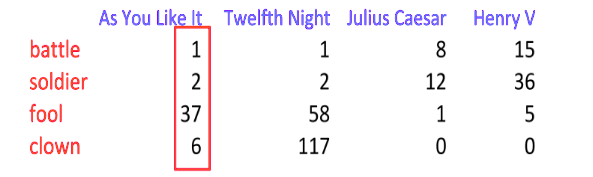
\includegraphics[scale=0.30]{image/doc-word.png}
	\end{minipage}
	\begin{minipage}[b]{0.47\textwidth}
		\centering
		\caption{Term-Context Matrix}
		\label{word-word}
		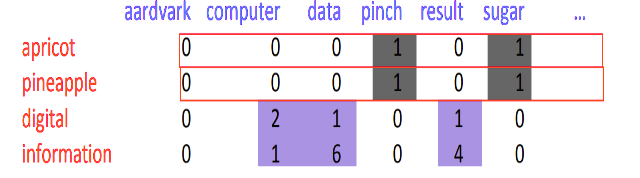
\includegraphics[scale=0.30]{image/word-word.png}    
	\end{minipage}
\end{figure}

Term-context matrix was introduced to handle this limitation and measure the similarity between words.  It used vocabulary words as its columns as well as its rows. Given the size of the vocabulary $|V|$, the term-context matrix carries the word co-occurrence count, within a specific window size,  with a dimension $|V| \times |V|$ as shown in Figure \ref{word-word}. These representations are also called Sparse Vector Representations as most of the matrix cell values are zero. They mostly capture syntactic information rather than the semantics of the word as the window size gets smaller. The difference in orientation of two vectors denotes the measure of similarity between words. Usage of a sparse vector model for any semantic analysis task was computationally complex. To overcome this issue, many models were proposed to generate short and dense representations as: 1) dimensionality reduction using singular value decomposition; 2) neural network approaches like skip-gram and Continous Bag of Word (CBOW). In this project, we will focus on the models that use neural networks for creating words and sentence representations, as the latter method is more computationally efficient than the former approach \citep{jurafsky2014speech}.

\section{Machine Learning models}

The learning theory and pattern recognition in AI gave rise to the field of machine learning \citep{jurafsky2014speech}. The main objective of the machine learning algorithms is to learn from the previous data and predicts future data based on its previous knowledge. It learns a hypothesis consisting of weight parameters, which map the input features to output or target values. For any training set with input and output $\{(x_{i},y_{i})\}_{i=1}^{n}\}$, these algorithms learn a model \textit{h(x) = y} from a collection of statistical feature set, extracted from the input in the training dataset. Then, it makes predictions on the unseen data.  While training , the parameters are optimized based on an error rate of training time output $\bar{y_{i}}$ against true output $y_{i}$, for \textit{k} features $<x^{1}_{i},x^{2}_{i},..,x^{k}_{i}>$ extracted from the input $x_{i}$. The data with discrete outputs such as RTE tasks are segregated as the classification problem, and  the data with the continuous value output such as sentence relatedness, are classified as Regression problem. 

\subsection{Traditional ML models}

In this project, the ensemble of machine learning algorithms such as Support Vector Machine, Random Forest, and Gradient Boosting, is used for learning an RTE classifier and a sentence relatedness task-based regressor. 

\begin{figure}[!tbp]
	\centering
	\caption{A simple Decision Tree}
	\label{tree}
	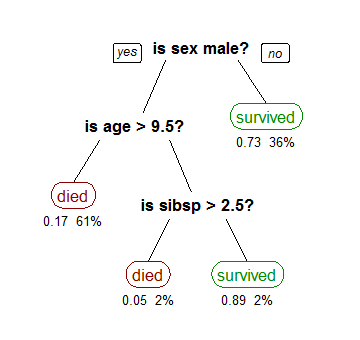
\includegraphics[scale=0.50]{image/tree.png}
\end{figure}


Random Forest is an ensemble classifier that consists of a collection decision trees. Decision Tree is a tree with leaf and decision nodes that represent the function that takes a vector of feature values, and outputs a single target value. The output value can be discrete or continuous. It decides the prediction based on a specific sequence of rules. Each internal node corresponds to a condition applied to the training set, using any one of the input features, that splits the data as shown in Figure \ref{tree}. Although decision tree performs well, it is prone to over-fit as the decision node rules are built from the distribution of the training data. Therefore, it does not generalize well on the unseen data while testing. But, Random forest does not over-fit as it is an ensemble of decision trees, constructed from the sub-samples of the training data as shown in Figure \ref{rf}. 

\begin{figure}[!tbp]
	\centering
	\caption{Random Forest}
	\label{rf}
	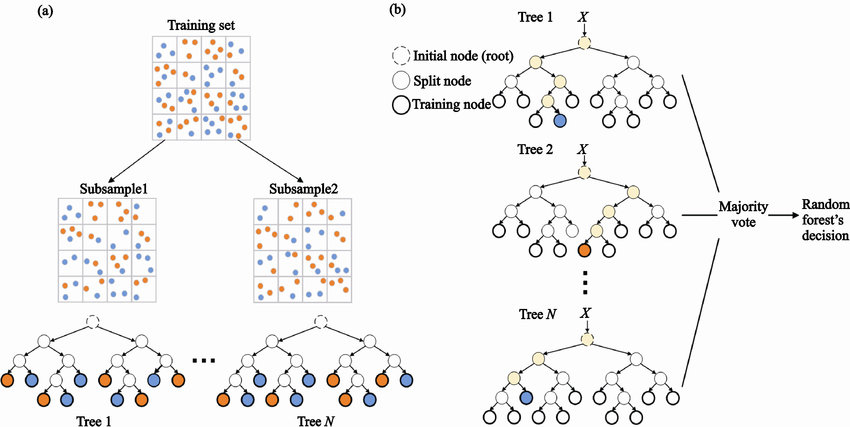
\includegraphics[scale=0.40]{image/rf.jpg}
\end{figure}

Support Vector Machine (SVM) algorithms apply to both linear and non-linear data. It is one of the most popular robust algorithms which performs well even with the small quantity of data .i.e with less prior knowledge about the problem domain. The critical trick that contributes to its robustness is maximum margin separator, a decision boundary with the most significant possible distance between the hypothesis and the training data points. This decision boundary helps the model to generalize well on unseen data. SVM handles linearly non-separable input data points, by expanding the hypothesis space, by transforming the input data into higher dimensional space. The data points are projected to a higher dimension using a kernel function. In higher dimension, a linear separating hyper-plane is created using kernel function to classify the input data with its class label. This separating hyper-plane is a non-linear line in the original space. 

Boosting algorithm is an ensemble of a set of learning algorithms that combines many base models that have limited prediction ability. Initially the boosting algorithm focused on binary classification $c(x)= sin(f(x))$ with response $\bar{y} \in \{-1,1\} $ where  

\begin{align}
f(x) =     \sum_{i=1}^{N} \varTheta_{i} c_{i}(x)
\end{align}

and $c_{i}$ are the base learning models,

The boosting algorithm learns the model by assigning weights $\varTheta$ to the data and training the weak classifiers against the weighted data-set. At each iteration, the weights are optimized in a way that the mis-classified data points get higher weights.

Performance of all these algorithms crucially depends on the features selected to represent the sequence. For example, choosing feature/attributes such as pos-tags proportion, syntactical structure equivalence, and word taxonomy etc. to train a model for STS task would obviously give a better performance than a model trained on only the word count feature. The extraction of each attribute takes a long time and finding the interactions between this feature, specifically for a task further slows down the training process. Most of the time, the model is provided with n incomplete or over specified feature set. If an algorithm can learn the attributes by itself, the training process can be automated more efficiently, and it helps in solving many NLP tasks. Neural networks are one such algorithm which can learn the feature on it own.

Since 1980, various neural models have been proposed. Initially, neural models did not perform well in any task as they learn the feature by itself and require an enormous amount of data to generalize for unseen data. Recent insights in optimization, advances in parallel computing, and the availability of large datasets encouraged these architectures to achieve state of the art performance. 


\subsection{Neural Networks}

A neural network is a directed graph with neurons as its node. Neurons are computational units connected by directed links. Each link has a weight that determines its importance or strength. Similarly, all the computational units consist of activation functions that are applied to the input. The activation function can be any linear or non-linear function such as sigmoid $(\sigma)$, hyperbolic tangent (tanh), and rectified linear units (RELU) etc. So, an output of any computational units is a function over the sum of the weighted inputs. Consider a computational units with activation function $f$ that takes inputs $x_{1},x_{2},...,x_{n}$ with weights $w_{1},w_{2},...,w_{n}$ and bias $b$ as shown in Figure \ref{neuron}. It is formally expressed as:

\begin{figure}[!tbp]
	\centering
	\caption{A simple neuron}
	\label{neuron}
	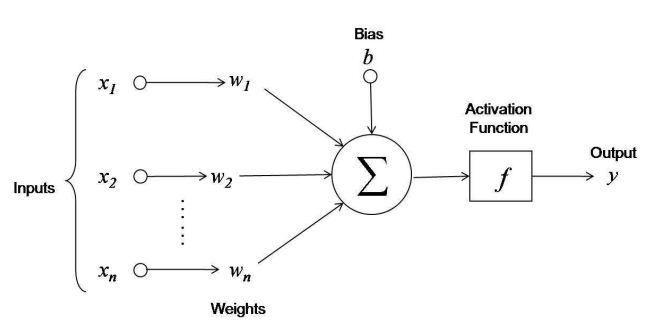
\includegraphics[scale=0.50]{image/neuron.jpg}
\end{figure}

\begin{align}
z & = \sum_{i=1}^{n} wx_i + b \\
y & = f(z)
\end{align}


 A simple neural network with two inputs $a$ and $b$, one hidden unit $c$, and an output unit $d$, is visualized as shown in Figure \ref{net}. Consider a sigmoidal function as the activation function in node $c$ and $d$. This network can be trained by optimising its weights $[W_{ac}, W_{bc}, W_{cd}]$ based on an objective function. The training has two phases: forward pass and backward pass.



\begin{figure}[h]
	\centering
	\caption{Neural Network}
	\label{net}
	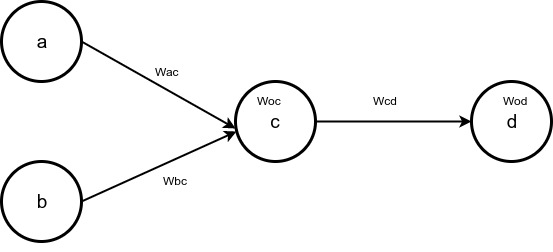
\includegraphics[scale=0.44]{image/Trace_Back_Prop.jpg}
\end{figure} 



\subsubsection*{Forward Pass}

For node c, $in_{c}$ is computed from the given weights and the input. The $in_{c}$ is fed into the activation function to get the output $A_{c}$. The output $A_{d}$ of Node $d$ is computed in the same way.
\begin{align} 
in_{c}    & = W_{ac} \times a + W_{bc} \times b + W_{oc} \\
A_{c} & = \frac{1}{1+exp(-in_{c})} \\
in_{d}    & = W_{cd} \times A_c + W_{od} \\
A_{d} & = \frac{1}{1+exp(-in_{d})} 
\end{align}

%For Node d, $in_{d}$ is computed from the given weights and the output $A_{c}$ of the previous node c. The $in_{d}$ is feed into the activation function to get the output $A_{d}$  
%\begin{align*} 
%
%\end{align*}

\subsubsection*{Backward Pass for weights adjustments}
The total loss of the networks is computed using the objective function $L = \frac{1}{2} (y - A_{d})^{2}$, where y is an actual output and $A_{d}$ is the predicted output. The gradient of loss $L$ is calculated concerning all the weights.

For example, gradient of loss computed with respect to $W_{cd}$, 

\begin{align*} 
\frac{\partial L}{\partial W_{cd}} & = \frac{\partial L}{\partial A_{d}} \times \frac{\partial A_{d}}{\partial in_{d}} \times \frac{\partial in_{d}}{\partial W_{cd}}    \\
& = \delta_{d} \times  \frac{\partial in_{d}}{\partial W_{cd}}  \\
& = \delta_{d} \times  \frac{\partial ( W_{cd} \times A_c + W_{od})}{\partial W_{cd}}
\end{align*}
\begin{align}
& = \delta_{d} \times  A_c
\end{align}  
% the rate of change of loss (gradient) \textit{with respect to} all the weights are calculated. 
where $\delta_{d}$ is a modification error. Weights are updated based on the gradients as shown below.
%The weight update rule in between layers i and j are 

\begin{align} 
W_{c,d} \leftarrow W_{c,d} + \alpha \times A_{c} \times \delta_{d}
\end{align}

where $\delta_{d}$ is a modification error,

%\begin{center}
%    
% gradient of Loss w.r.t $A_{d}$ $\times$ gradient of activation output $A_{d}$ with respect to $in_{d}$.
%\end{center}

If there is more than one output unit in the layer, the partial derivative of the error across all of the output units, is equal to the sum of the partial derivatives of the error concerning each of the output units.

A simple feedforward neural accepts fixed length input, and the length of the sentences are varying. To feed a sequence as an input, the vector representations of each word in the sentence should be transformed using additional operations such as average or sum. By changing the sequence input, it is impossible to capture word order information. Recurrent neural networks handle this case by employing recursive computational units as per the sequence length.
%Earlier, neural models proposed used have many hidden layers as it approximates any function.

\section{Word Vector Representation}

Firth's hypothesis of representing each word meaning by using its nearby words, was successfully used in many statistical NLP techniques. For instance, Brown Clustering \citep{brown1992practical} , Latent Dirichlet Allocation \citep{blei2003latent} etc used word co-occurrence count as its primary component. In the field of deep learning, \cite{bengio2003neural} proposed a language model based on a neural network that predicts the next word for the given previous words in a sequence. They also noticed that this prediction model helped in learning a vector representation for words called word embeddings or word representations.
%The representations were learnt by starting with the random vectors and shifting its vector closer to the vector of its similar words throughout the training process\footnote{wrong. The vector moves close to words with similar meaning. }. 
Later in 2008, \cite{collobert2008unified} showed the usefulness of word representations in various downstream NLP tasks.
%the efficient use of pre-trained word vectors in different work was explained by. 
Inspired by these models, \cite{mikolov2014word2vec} proposed two novel methods: 1) Skip-Gram with Negative Sampling (SGNS); 2) Continous Bag of Words(CBOW) models for learning word representations. The SGNS model is discussed in detail below, as it is widely adopted and used as an input for many sentence representations model \citep{kiros2015skip}.
%objective has been adopted by a sentence representation model and made an important contribution to learn a generalizable sentence representation. This model was demonstrated to be inexpensive compared to previous models and performed very well in capturing the general syntactical and semantic information. The training objective of these models is to learn word vector representations that are good at predicting the surrounding words. The detailed architecture of the skip-gram model is shown in figure \ref{skipgram}. 

\begin{figure}[!tbp]
	\centering
	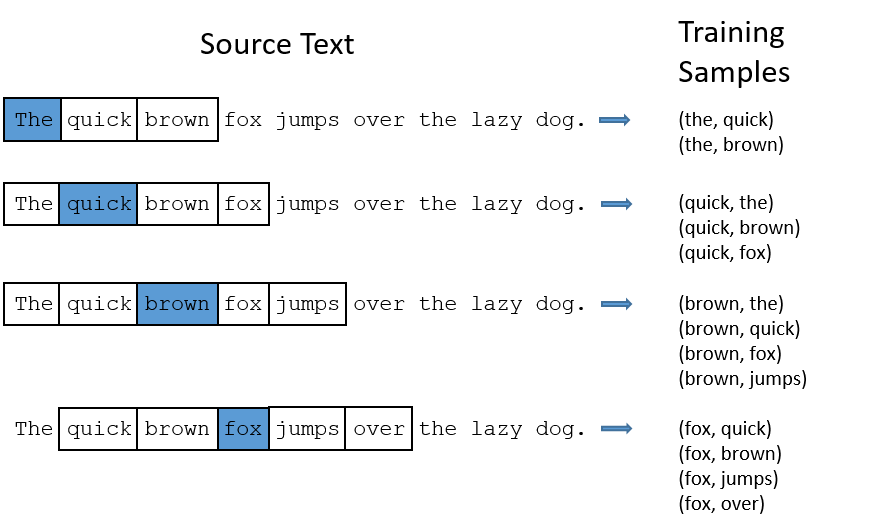
\includegraphics[scale=0.70]{image/train_samples.png}
	\caption{Training samples for skip-gram - Words pairs from raw corpus}
	\label{train_sam}
\end{figure}

%The primary goal of the skip-gram model is to learn the weights of the hidden layer which transforms to the word vector representation undergoing the process of training.\footnote{ The goal of skip gram was just to predict word based on context. You just said this in the last sentence.} Given any word in the vocabulary $V$ from a training corpus, skip-gram model outputs a probability that determines how likely the words in the vocabulary can appear near to the source word.\footnote{Third time same concept in different words} 

\begin{figure}[h]
	\centering
	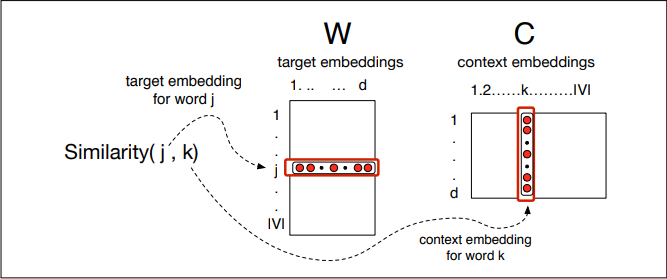
\includegraphics[scale=0.50]{image/cbows.png}
	\caption{Context and Word matrices \citep{jurafsky2014speech}}
	\label{C_W_matrics}
\end{figure}


The SGNS model was trained on a monolingual text corpus, where every centre word is used to predict the surrounding words within a window size as shown in Figure \ref{train_sam}.
%using samples consisting of word pairs derived from raw text corpus with defined window size as shown in Figure.
The model takes word input in the form of the One-Hot vector of dimension $1\times|V|$. While building the vocabulary from the training corpus, One-Hot vector $1\times|V|$ gets assigned to each word consisting of value 1 in the position that is the same as the position of the word in the vocabulary, and value 0 in all other positions. This input vector X is multiplied with the word matrix $W$, to get the hidden layer $v$ (target word representation) of dimension $1\times|D|$, where D is the dimension of a word representation. The dot product of the hidden layer and the context matrix is to find the context word score as shown in Figure \ref{C_W_matrics}. For each word, the context word score is normalized using soft-max function, to get the probability of each word in the vocabulary occurring near the given the word. For a word $w_{j}$, the probability of any $k^{th}$ word in V is calculated as shown in equation \ref{eq1}

\begin{align}
\label{eq1}
p(w_{k} | w_{j}) = y_{k} = \frac{\exp( c_{k} \cdot v_{j})}{\sum_{i=1}^{|v|} \exp(c_{i} \cdot v_{j}) } 
\end{align}


The output of the network is the vector $1\times|V|$ consisting of the probability distribution of each word in the whole vocabulary. Each probability value in the vector position denotes the likelihood of a word corresponding to the same position in the vocabulary. Cost function $L$ tunes the weight parameters in this network by using equation \ref{eq2}
\begin{align}
\label{eq2}
L = - \log ( p(w_{O,1}, wO,2, . . . , w0,C|wI))
\end{align} 


The derivative of $L$ with respect to input units of the output layer and hidden layer, constitute the prediction error. The learning algorithm is started with the randomized word and context matrices (weight parameters of this network). Optimizer algorithms such as Stochastic Gradient Descent are used to tune the weight parameters using error back-propagation to broadcast the gradient through the network. Later, the Skip-Gram model was improved by replacing the soft-max function in the output layer with Negative Sampling. This model provided state of the art performance while testing for semantic and syntactic word similarities. \citep{mikolov2014word2vec}. 


\begin{figure}[!tbp]
	\centering
	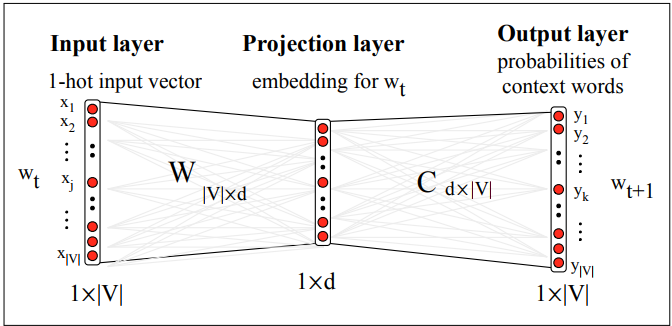
\includegraphics[scale=0.50]{image/skip-gram.png}
	\caption{Skip-gram Model \citep{jurafsky2014speech}}
	\label{skipgram}
\end{figure}

\section{Sentence Representation Model}
As word representation models became very useful and predominantly used, a natural next step was to extend such approaches to build sentence encoders. The main objective of sentence encoders was to learn an accurate sentence representation that would capture its semantics using previously trained word representation.
%As the models proposed for learning word representations are well-established models and proved to be successful in their performance; recent research has focused models that can learn a general sentence representations that would capture its proper semantics using previously trained word representations. 
The vector representations can be learned by using two approaches 1) Supervised models \citep{conneau2017supervised} 2) Unsupervised models \citep{kiros2015skip}. Skip-gram model is unsupervised learning as its objective function was to optimise the word representations. In this type of learning, general information is captured. The knowledge obtained by these models can be transferred to any NLP task that needs to process a sequence. 


Supervised learning of vector representations is training a model on a pre-defined task, with defined input-output samples where the model parameters are optimised based on the task. The word representations are learned in internal states as the model is trained on an STS task. In this type of learning, the model learns the information that is specific to the task and fails to capture general knowledge. All proposed models aim to generate an accurate and generic sentence representation that consists of the whole meaning of the context. These generic representations are vital as they can be used for various tasks with minimal adaptation. This property results in the smooth transfer of learning to the model that learns any specific task. By promoting Transfer Learning, the training complexity and training time for particular tasks, decreases.  

%\subsubsection{STS Features and Accurracy}
%
%For STS task, traditional machine learning algorithms used handcrafted features from the raw sentence such as word overlap, knowledge based similarity, length features and other similarities. Neural models use word representation to train the models. Recently neural models \cite{conneau2017supervised} \citealp{kiros2015skip} \cite{shao2017hcti} have been popular as they outperform all the traditional machine learning algorithms. Ensemble techniques which combine the prediction techniques of traditional machine learning models and neural models are also being explored.
%
%
%The performance of the model is measured using Pearson Correlation of the predicted score with a human judgment score given in the dataset \citep{agirre2015semeval}. Generally, correlations measure the extent to which two variables change together. Pearson Correlation, meaures the direction of linear relationship between pairs of continous variables that are well suited for the sentence relatedness task.
% 


\chapter{Related Work}


Despite developing a number of learning algorithms for representing words and sentences, generating high quality and efficient sentence representations remains an unsolved problem \citep{conneau2017supervised}. An efficient sentence representation that consists of the whole meaning with context is important as it can be used across various tasks with minimal adaptation. This property results in a smooth transfer of the learning to train any NLP task. We focus on the STS task, as \cite{conneau2017supervised} demonstrated that natural language inference tasks appear to capture more generalizable sentence representation using Transfer learning. This chapter discusses the existing models and comparison studies in order to compare and study different models used for STS tasks and to infer how they impact in learning good sentence representations.

\section{Traditional Machine Learning Models}

For decades, traditional machine learning algorithms such as support vector machine or logistic regression were to used to solve any NLP tasks. In 2012, supervised models based on the lexical and syntactic features of the sentence pair, showed promising results on measuring semantic relatedness. These systems gave 52\% - 59\% correlation on various data-sets by using regression models consisting of various similarity measures as its input features. The unsupervised models did well for next two years in row using the WordNet knowledge and the LSA similarity measures which assume that the words with closer meaning highly co-occur in the text corpora. 

\cite{han2013umbc_ebiquity} proposed three approaches that involved 1) LSA similarity model, 2) semantic similarity model based on the alignments quality of the sentences, and 3) support vector regression model that had features from different combinations of similarity measures, and the measures from two other core models. It was observed that using the n-gram overlap feature increased LSA similarity model. Out of three models proposed by \cite{han2013umbc_ebiquity}, the alignment based system gave 59\% - 74.6\% Pearson Correlation on four different data-sets. Using this model's alignment quality as one of the features in the Support Vector Regression model improved the correlation score to 78 \%.  Various supervised models using uni-gram (one word) or bi-gram (two words) overlap, vector distance, and cosine similarity of sentence embedding, were proposed \citep{agirre2015semeval}.   

\cite{tian2017ecnu} proposed a system that adapted ensemble learning techniques to solve the Textual Entailment and STS tasks, using the same set of features. The combination of classical NLP models like Support Vector Machine, Random Forest, Gradient Boost and a deep learning model are used in this system. For classical NLP models, single sentence and sentence pairs feature sets, are hand engineered based on properties like N-gram overlap, syntax, alignments, word sequence, word dependency, word representations etc.. In SEM-EVAL 2017, this mixed ensemble model gave 81 \% Pearson Correlation, outperforming all the neural models presented in that shared-task event.

Although using hand-crafted features in the above mentioned models works, it has some drawbacks such as tuning the features extracted on addressing the corpus from new domains, high computational complexity in hand engineering the features, and effective feature selection etc.. Recent approaches in deep learning continue to prove that the problem of semantic text matching can be handled in an efficient way \citep{cer2017semeval}. The problem of semantic word matching can be extended to solve the problem of the semantic sentence match by using deep learning approaches. This helps when it comes to effectively learning the word meanings in the sentence individually and deriving a meaningful sentence representation from the word vectors.  

\section{Neural Models} 

This section discusses the top ranking neural models presented in Sem-Eval 2017 that have been proposed to build sentence representations and predict sentence relatedness.

\cite{kiros2015skip} proposed the Skip-Thought model based on skip-gram objective from \cite{mikolov2014word2vec}. For any three consecutive sentences in the document $S_{i-1}, S_{i}, S_{i+1}$, the Skip-Thought model predicts the previous sentence $S_{i-1}$, and next sentence $S_{i+1}$ given any sentence $S_{i}$.
This work focuses on training an encoder-decoder model. A variant of recurrent networks consisting of gated recurrent units (GRU) \citep{cho2014learning} is used as an encoder to map input sentences into a generic sentence representation. RNN with conditioned GRU is used as a language model to decode the sentence representation and predict surrounding sentences $S_{i-1}$ and $S_{i+1}$. In evaluating a semantic relatedness task, Skip-Thought outperformed all systems proposed in a shared task SemEval 2014 \citep{marelli2014semeval}.
%and was outperformed by dependency Tree-LSTM model.

\cite{tai2015improved} proposed a recurrent neural networks(RNN) with tree based LSTM units with two variants Child-Sum Tree-LSTM and N-ary Tree LSTM. Given a sentence syntactic structure in a form dependency tree of the words, Tree-LSTM networks are capable of integrating the child node's information. The Tree-LSTM units in each node t consists of input gate $i_{t}$, output gate $o_{t}$, a cell unit $c_{t}$ and a hidden output $h_{t}$. Unlike Standard LSTM, the parent node has one forget gate $f_{tk}$ for each child node \textit{k} in the Tree-LSTM. This property allows selective usage of child information. Previously proposed RNN models with sequential LSTM units, have limited ability to capture the meaning difference in the two sentences raised due to word order and synactical structures. Tree-LSTM addresses this issue by computing its hidden layer output as a function of the outputs from its children hidden units and input vector. 

In modelling semantic relatedness, the input $x_{t}$ denotes the word vectors of the sentence parse tree. The proposed model retains the information of more distant words from the current words compared to other existing models. These properties make the model effective in highlighting the semantic heads in the sentence. It also captures the relatedness of two phrases which have no word overlap. With these properties, Tree LSTM performs better than existing sequential RNN-LSTM models, and models with hand engineered features on predicting the semantic relatedness of two sentences. But one major downside is that the dependency tree-LSTM relies on parser for dependency tree input, which is computationally expensive to collect and does not exist for all languages making it inefficient in cross-lingual sentence representations.



\cite{shao2017hcti} presented a simple Convolutional neural network model for STS tasks. This model constsis of CNN model and fully connected neural network (FCNN). CNN takes pre-trained word vectors from Glove \cite{pennington2014glove} enhanced with handcrafted features as its input. It enhances word vector to task specific forms in the convolutional layer, and max-pooling generates the task-dependent sentence representation. FCNN generates the similarity score ranging from 0-5. This model ranked 3rd in SemEval-2017 with a 78 \% correlation on STS tasks. 


\cite{pagliardini2017unsupervised} proposed a simple unsupervised objective Sent2Vec, to train a generic distributed representation for sentences. The main contribution of Sent2Vec is its low computational cost for both training and inference, relative to other existing state-of-art models. This model is an extension of CBOW training objective from Word2Vec \citep{mikolov2014word2vec}, to sentence context.


\cite{conneau2017supervised} investigated the performance of various supervised encoders in learning universal sentence representations. They hypothesized that textual entailment task is a good choice for learning universal representations and demonstrated the hypothesis with various encoder models. To prove that the sentence representations learned are universal, the representations learned from unsupervised and proposed hypothesis was used in 12 different transfer tasks, such as Caption-Image retrieval, Paraphrase detection, Entailment/semantic relatedness, and sentiment analysis etc.. As the result of their experiments, Bi-LSTM with max-pooling trained on Natural Language Inference Task (Textual Entailment), generated the best sentence representations, and outperformed SkipThought \cite{kiros2015skip} and FastSent \cite{hill2016learning}.

\chapter{Modeling Sentence Encoders}

In recent times, a wide variety of encoders for learning sentence representation have been proposed by NLP researchers. However, there is a lack of understanding about the characteristics of different encoding techniques that can capture useful, accurate semantic information \citep{conneau2017supervised}. In feature based machine learning models, hand crafting and selecting optimal features is hard. Although neural models learn the feature by itself, they suffer from an inherent bias toward the task and data-set that they are trained on.
%captures the bias in the dataset effectively. 
This feature is a downside because it learns the task very well and fails to capture generic useful information during the training time, leading to poor generalization. On the contrary, neural models trained independent of any task give more importance to general information. But, it fails to specialize the model for any specific task. 

Many factors affect how the basic semantics of a sentence are being captured during training. An important factor to note is the task for which the model is trained. Similarly, the encoders' architecture for both task dependent and independent neural models also impacts learning in different ways. This comparison study on these encoder's architecture and performance on STS task primarily focus on understanding for following:

\begin{itemize}
	\item Encoder's ability to capture semantics.
	\item Encoder's potential to capture accurate meaning representations that is generic.
\end{itemize}	

Above two objectives of this comparison study answer the following question that helps in improving the models that already constitute the state of the art in sentence encoding.

\begin{itemize}
	\item What are the features that contributes more to the prediction while using traditional machine learning models ?
	\item What are the trade-offs incurred by neural networks as opposed to the traditional machine learning models?
	\item What is the impact of various activation functions used in the encoders hidden layers?
	\item What is the preferable neural network architecture for learning better sentence representations? 
	\item What is the impact of various optimizers in training a model?
	\item Since the dimension has direct effect on the memory requirements and processing time, where dimension has a good trade-off between accuracy and training time? 
\end{itemize}

We perform a systematic comparison of different encoder techniques and assess their ability to capture semantics of the sentence, based on their performance in STS tasks. To investigate the performance, various models such as support vector machine (SVM), Random Forest (RF), Convolutional Neural Network Encoder \citep{shao2017hcti} and BiLSTM RNN with max-pooling \citep{conneau2017supervised} were implemented. These encoder models achieved good accuracy in predicting sentence relatedness, and it outperformed the state-of-the-art encoders such as SkipThough, and FastSent while being much faster to train than others. The neural models were implemented using the Pytorch and keras library. The ensemble model was implemented using Sci-kitLearn library. \cite{conneau2017supervised} demonstrated that Recognizing Textual Entailment (RTE) captures semantics very well. Based on this inference, the neural models were trained using data-set from Standford Natural Language Inference (SNLI) corpus  \citep{bowman2015large}, and Sentences Involving Compositional
Knowledge (SICK) corpus \citep{marelli2014semeval}, for semantic relatedness and RTE tasks.
 

\section*{Learning Methods}
%	\subsection{Feature Engineering}
This section describes the architecture of a various learning methods that are investigated for its ability in extracting sentence representation. 

\section{Ensemble Model}
\label{ensemble}

	This section discusses about the architecture details of an ensemble model proposed by \cite{tian2017ecnu}. This model adapts a combination method to intergrate the prediction of traditional ML algorithms such as support vector machine (SVM), Random Forest (RF), Gradiant Boosting (GB) and a neural network algorithm such as deep averaging network. This project explores the combined performance of SVM , RF and GB as mentioned in \citep{tian2017ecnu}. Given \textit{n} training data with input and output $ \{(x_i,y_i)\}^{n}_{i=1} $, these models focus on estimating a function (hypothesis) \textit{h(x)=y} that maps input to output. In STS task, with sentence pair as the input, a standard approach is to represent the sentence pair in the form of similarity features. Therefore,  effective feature representations that capture semantic and synactic matching degree are hand engineered. 
	
	With these feature representations as input, the predictions are done based on the hypothesis \textit{h(x) = W . X} where X is the similarity feature vector and W is the corresponding weight vector.  The model learns an appropriate weight for each feature while training. In Ensemble approach, various models trained on sentence relatedness task with continous outputs, are optimizied based on the average of the score returned by them. In the case of classification tasks such as RTE, the models are optimised based on the majority voting of their classifications. The architecture diagram of this model is shown in Figure \ref{ensemble}.
	
	\begin{figure}[!tbp]
		\centering
		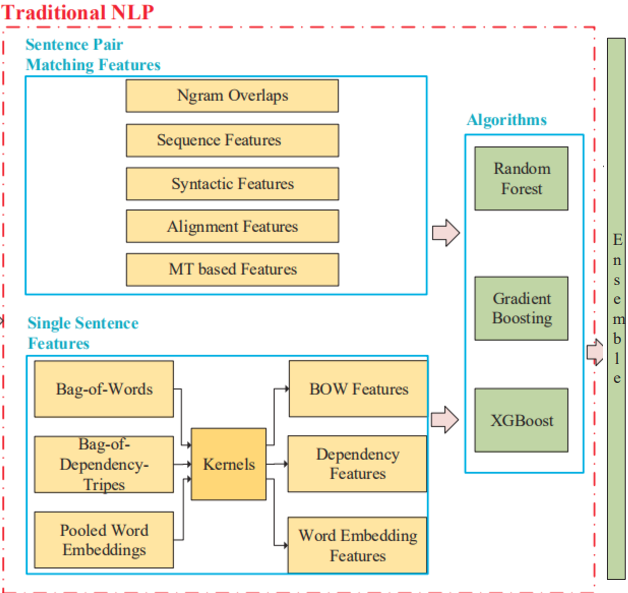
\includegraphics[scale=0.40]{image/Ensemble.png}
		\caption{Ensemble Model \citep{tian2017ecnu}}
		\label{ensemble}
	\end{figure}
	
	\subsection{Features}
	For this ensemble model, the features of a sentence pair is extracted based on the length of two sentences, n-gram overlap, syntactic structure, alignment and machine translation metrics. N-Gram represents the group of \textit{n} consecutive character/words/sequence in a corpus. For the STS task, the  sequence of words or phrase overlaps are useful in expressing the common expression between two sentences. In this project, the normalised n-gram overlap is extracted in both word and character level. Similarly the longest common sub-sequence, prefix and suffix are computed to extract the sequeunce similarity. To estimate accurate similarity, the words are lemmatized where the words are replaced with its root word. 
	
	Although the sequence of words overlap information can give a good indication of similarity, it fails to capture the word dependencies in a sentence which primarily influence the sentence meaning. The syntactical structure of a sentence is captured in the form of tree and the number of common subtree, constitutes the feature set. Further, the monoligual word alignment proportion is extracted as a feature. This feature maps the words between two sentences based on their meaning, parts of speech tag, and the synactic structure. The alignment features include normal alignment proportion, pos tag based weighted proportion. Other features include various WordNet based and word vector representation based similarities measures, such as
	
	\begin{itemize}
		\item \textbf{Levenshtein distance} : It signifies the number of minimum edits required to convert one sequence to the other. This is also known as Path distance. This feature  implies the sequence is more similar when the distance is shorter. 
		\item\textbf{Leacock-Chodorow distance} : This feature extends the path distance by scaling it using depth of hierarchy structure based on \textit{is-a } relationship
		\item \textbf{Resnik distance} : This feature measures the similarity based on taxonomy information of two words/sequence. The similarity is computed based on the distance of first common predecesor of the two words/sequence in WordNet's taxonomy tree which conveys how much two words are related.
		
		\item \textbf{Jiang-Conrath distance} : This feature is the measure of increase difference in relation of two words/sequence.  
		\item \textbf{Cosine distance} : Given the vector representation of words, normalised dot product of two vectors indicates the similarity between them.
	\end{itemize}
	
	Finally, a sentence pair is represented using 47 features. These features are standardised to [0,1] using max-min normalization to reduce the standard deviation and handle the outliers in the features. Then, the traditional machine learning models such as Support vector machine (SVM), Random Forest(RF), and Gradient Boosting (GB) are trained using these features.
	
	\subsection{Learning Models}  
	
	For semantic relatedness task, a list of sentence pairs $X =$ \{($S_{a1},S_{b1}$),.., ($S_{aN},S_{bN}$)\} is given as input. The sentence pairs come with similarity scores $Y$ = \{$Y_{ab1}, Y_{ab1},...., Y_{abN}$\} that consist of value ranging from 0 indicating no similarity to 5 indicating the high similarity between the sentences. The goal is to build a model that is able to produce the correct similarity score $Y_{ab}$ for each sentence pair \textbf($S_{ai},S_{bi}$).
	
	Formally, the task to learn is represented as,
	
	\begin{align} 
	h(w,f(S_a,S_b))  & \rightarrow Y_{ab} 
	\end{align}
	
	where function $f$ maps sentence pairs to a vector
	representation, in which each dimension expresses a certain type of
	similarity between the input sentence pair such as lexical, syntactic, semantic etc. The weight vector,
	$w$ is a parameter of the model that is learned during the training and $h$ denotes the STS prediction model.
	
	The RTE task is a classification problem that consists of three target clasess  \textit{ C =\{entailment, contradiction, neutral\}}. A classifier function $\gamma$ is learned to map the sentence pair to its corresponding RTE class labels \textit{C}.
	
	In ensemble of SVM, RF and GB, their predictions are combined into one final prediction using the Stacking algorithm. In stacking, the training set is split to several subsets and each model is trained and tested on one of those subsets. Finally the predictions are fed into an outer model with their actual target value for its training. This outer classifier combines the prediction of SVM, RF and GB.
	
	
\section{Convoutional Neural Network}
	This section explains the convolution neural networks (CNN) based learning model used for semantic sentence similarity. The two main components of this model are (CNN) based sentence representation model, and fully connected neural networks (FCNN) used for STS task. The CNN architecture consists of two convolution networks that work parallel to mapping the two sentences to a vector space. The vectors of the sentence pairs are used by FCNN to classify their sentence similarity score. In the following, we first describe our sentence model for mapping sentence pairs to their intermediate representations and then explain how these representations are used to classify the relatedness score.
	
	\subsection{Sentence Model using CNN}
	CNN architecture for mapping sentences to
	vector representations inspired from \cite{shao2017hcti} is shown in Figure 4.2. This architecture consists of two 1-dimensional convolution layers and a max pooling layer. The objective of this network is to convert the raw sentence into vector representations from \cite{pennington2014glove}, using pre-trained 300 dimension word embeddings of all the words \{$w_{1}, w_{2},...,w_{|s|}$\} present in the sentence.
	
	The input sentence to the convolution layers is treated as a sequence of a real valued number where the real valued integers are retrieved from the integer-word mapping present in the vocabulary V. The vector representation of all the words $ w \in \mathbb{R}^{d}  $ are drawn from embedding matrix  $ W \in \mathbb{R}^{d \times |V|} $ in the embedding layer. To enhance the word representation with respect to this task, a true flag for word overlap is added as an additional dimension into the word vector representation for each word in the sentence. Then the CNN network applies the convolution and max pooling operation to find the optimal feature vectors for the sentence that capture its semantics. 
	
	The idea behind the convolution layer is to learn the features which identified the relationship between n-gram of the sentence using weight vectors \textit{m} $\in \mathbb{R}^{|m|}$ . The $1 \times 1$ weight vector \textit{m} also known as filters of the convolution is used. This convolution operation is followed by applying the Relu activation function to learn non-linear decision boundaries. This filters out the insignificant features learned in previous operation. The output from the convolution layer is passed to the max pooling layer with pool size (1, $|S|$) where the semantic information learned is aggregated, and reduces representation dimension from $1 \times |S| \times 300$ (word vec dimension) to $1 \times 300$ (word vec dimension). The convolution layers along with RELU activation function and max pooling acts as a non linear  feature detector for the given sentence. The output sentence representation from CNN is used to find the Semantic Difference Matrix by performing a series of operations on the two sentence vector. 
	
	\begin{figure}[!tbp]
		\centering
		\begin{minipage}[b]{0.43\textwidth}
		\centering
		\label{CNN_1}
		\caption{CNN Sentence Model \cite{severyn2015learning}}
		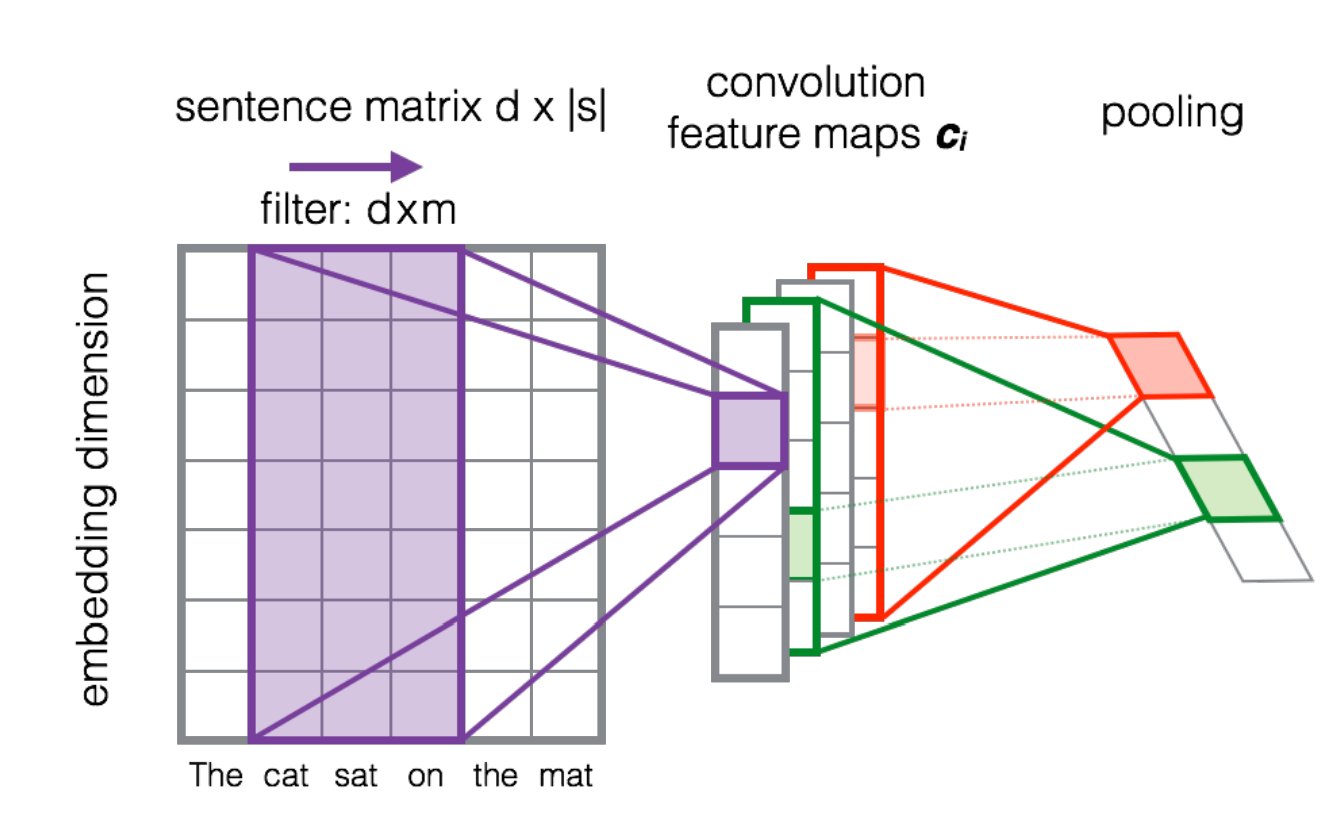
\includegraphics[scale=0.20]{image/CNN_sentModel.png}
		\end{minipage}
		\hfill
		\begin{minipage}[b]{0.40\textwidth}
		\centering
		\caption{Hyperparameters for FCNN \cite{shao2017hcti}}
		\label{params}
		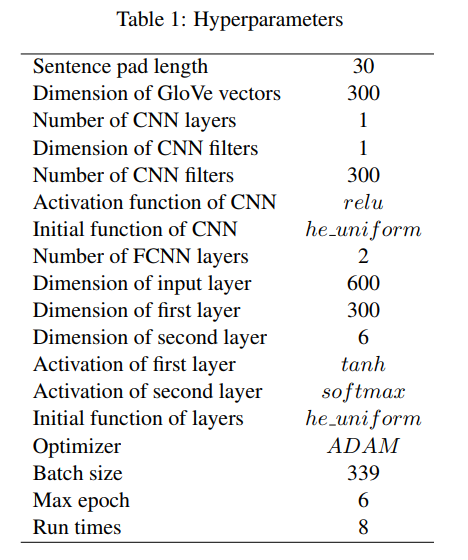
\includegraphics[scale=0.30]{image/hyperparameters.png}
		
		\end{minipage}
	\end{figure}
	
	
	\subsubsection*{Semantic Difference Matrix}
	The semantic difference matrix is generated by concatenating the vector difference and vector product of a two sentence representation. This matrix is used to classify the similarity measure using fully connected neural network (FCNN) with 2 dense layers. 
	
		\begin{align*} 
			SDV & =(|SV_{1}- SV_{2}|.(SV_{1} \circ SV_{2})) \\
		\end{align*}
	
	\subsection{Similarity Measure using FCNN}
	
	 This network consists of one hidden layer consisting of 300 computational nodes, and an output layer with 6 nodes. The hidden layer applies a \textit{tanh} activation function and the output layer applies softmax layer. The softmax layer calculates the probability over the six score labels. The hyper parameters of this network is shown in Figure \ref{params}.
	 The maximal point is calculated from the probability distribution over six score labels. Finally, the model is trained and optimised using the root mean squared loss of target and predicted continous value. 
	 
	 \section{Recurrent Neural Network}
	 This section desecribes the architecture of InferSent, a variant of recurrent neural network (RNN) proposed for RTE task \citep{conneau2017supervised}. This model outperformed all the existing state-of-the-art models such as SkipThought, FastSent etc, in extracting accurate sentence embedding. InferSent consists of a bi-directional Long-Short Time Memory (LSTM) based RNN sentence encoder and a fully connected neural network based decoder as shown in Figure \ref{bilstm}. The architecture of encoder is discussed in the following section. 
	 
	\subsection{Bi-LSTM with max pooling}
	Generally, RNN has the ability to accept input of arbitary length and return a fixed dimensional vector. Also, it is capable of propogating the previously processed input's information while processing a word in the given sequence at timestep \textit{t}.
	This encoder architecture consists of bi-directional RNN which reads the sentence in two opposite directions. It is capable of remembering the past and future context information of a sequence at any time step. The objective of this network is to extract generic sentence representation for a given word representations of the words present in the sentence.  
	
	
	\begin{figure}[!tbp]
		\centering
		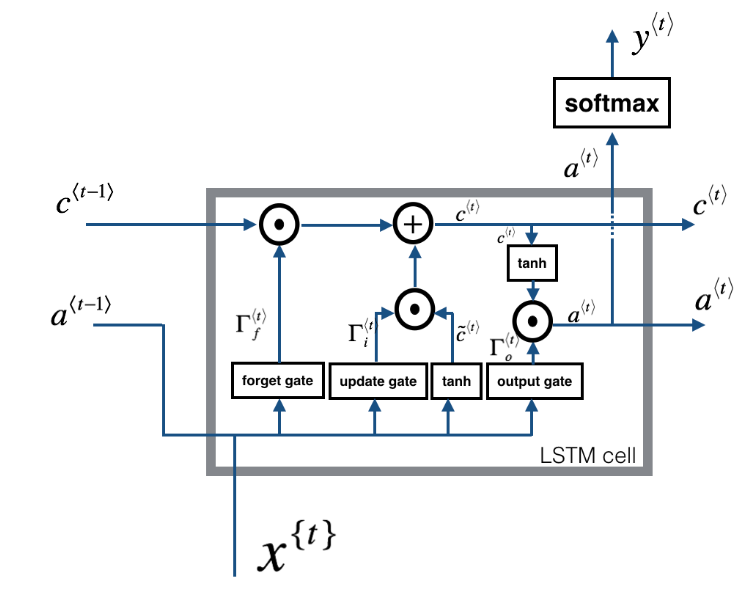
\includegraphics[scale=0.40]{image/LSTM.png}
		\caption{A Single LSTM cell \citep{SeqMod2018Andrew}}
		\label{lstm}
	\end{figure}
	
	 The RNN consisting of a sequence of LSTM computational cells in this architecture accpets a raw sentence $<x^{1},x^{2},...,x^{t}> \in S$ input in the form word representations. It reads the input \textit{S} and process one word $x^{t}$ at a time $t$ sequentially. Each LSTM cells consist of a memory cell $C$ to remember information about previous words and forget, update,output gates to manage memory while processing the words in the sentence. This helps LSTM to keep track of the synactical structure in the case where it stores a gender of the subject and relates it to the pronoun in the later part of the sentence. Each cell accepts current word input $x^{t}$ , memory cell $\overrightarrow{C^{t-1}}$ from the previous cell state and hidden state $\overrightarrow{a^{t-1}}$. It outputs a fixed dimension hidden state vector $\overrightarrow{a^{t}}$ and its prediction $y^{t}$ for current time step $t$. For this bidirectional RNN, the hidden state output $ a^{t} $ at each time $ t $ is computed by concatenating the hidden state output $ [\overrightarrow{a^{t}},\overleftarrow{a^{t}}] $ of forward  and backward LSTM cells . Max pooling is applied over the varying length hidden state outputs $<a^{1},a^{2},a^{3},...,a^{t}> $, to obtain a fixed length sentence representation. In Max pooling, maximum value over each dimension of the hidden states is selected to represent the input sentence.
	
	\begin{figure}[!tbp]
		\centering
		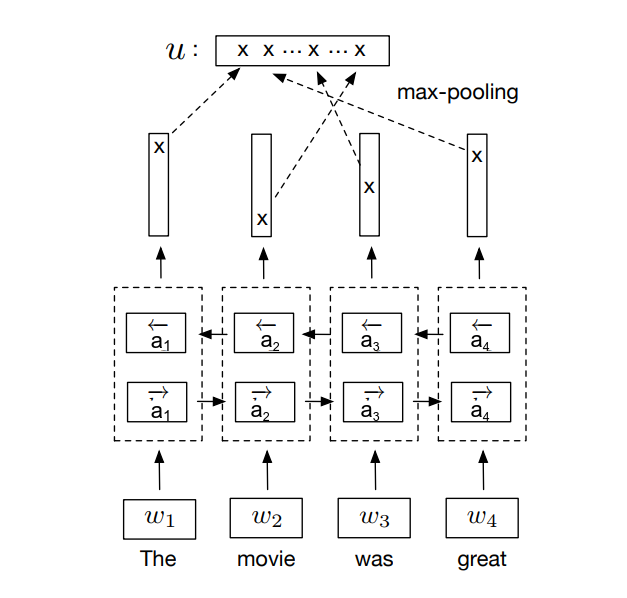
\includegraphics[scale=0.40]{image/Bi-LSTM.png}
		\caption{A Bi-LSTM Network \citep{conneau2017supervised}}
		\label{bilstm}
	\end{figure}
	
	\subsubsection{Semantic Difference Matrix}
	
	After extracting the sentence representation $\{u,v\}$  for the sentence pair $\{S_{1},S_{2}\}$, the semantic difference matrix is computed by concatenation, element-wise product and absolute element-wise difference of $u$ and $v$ as shown in equation 5.2 .
	
	\begin{align} 
	SDV & =([u,v],|u - v|,(u \ast v)) 
	\end{align}
	
	\subsubsection{Textual Entailment Classifier}
	
	This semantic difference matrix is fed into a fully connected neural network decoder to classify the textual entailment in the sentence pair. This network consist of a single hidden layer with 512 hidden units and a output layer with 3 output nodes. 
	
	The whole encoder decoder architecture is trained  and optimised using the categorical cross-entropy as its loss function. With the probabilties from the decoder's softmax layer, one hot vector is calculated by assigning 1 to the class with maximum probability and 0 to others. It is compared to the target one hot vector as its a multi-class classification while calculating loss.
	
	\section{Summary}
	In this chapter, the motivation and objective of the comparison study was discussed. Also, this chapter presented the architectural details of the models involved in the comparison study. Chapter 5 outlays the experiments and evaluations of these models.
	
	  
	 
\chapter{Experiments}

 In this chapter, we discuss the results of the comparison study. The goal of our study is to compare the ability of traditional machine learning and neural models in capturing meaning representations of sentences. All the models are trained on Sentence Relatedness and Recognising Textual Entailment (RTE) task. During training, the encoder model learns sentence representations that allows a decoder to judge how much two sentences are semantically similar or whether two sentences have meaning overlap. To perform better in these tasks, the encoder model should capture the compositional meaning of the given sentence. 
 
 In section \ref{performance}, the sentence encoders are compared and analysed for its performance in Sentence Relatedness and RTE task. In section \ref{parameter-tune}, experiments are performed to tune the parameter of encoder architecture and presents the optimal parameter under which it performs best compared to other parameter
 settings.
 
 The performance of the models on STS task is evaluated using accuracy of its prediction. The accuracy of the STS models is measured using Pearson correlation between machine generated semantic score and gold standards created using humans judgement. It helps in capturing the linear relationship between the predicted and target semantic score. This correlation value ranges from -1 to 1 where, 1 indicates perfect positive correlation and -1,0 indicates no or negative correlation.
 
 Although complex models give better accuracy, they take a long time to train. The major aim of any machine learning algorithm is to minimise the loss in the predicted value when compared to target value. The model is trained until the loss converges to its global minima. Various hyper-paramter impact the time taken by a model to converge. Sometimes, the learning algorithm consistently learns unnecessary features because the randomness in the training data points. In this case, the loss is always high and the model is said to have high bias. This model doesn't converge to the global minima resulting in underfitting. In contrast, starts to memorise the training data which is known as overfitting. At this point, the model's prediction on unseen data is comparatively very less.  Analysing the time taken by loss of the encoder models to converge to its local minima can help in finding a tradeoff between the training time and the model performance. 
 
 In addition, the sentence representations encoders are evaluated for its performance on generating a generic sentence representation that aids in transfer learning. This evaluation is carried out by using representations learned from training RTE task as input in sentence relatedness task and vice versa. Generic representations are expected to perform well in both tasks in terms of accuracy. This helps in training a task that do not have sufficient resource.  
 
 In this chapter, we evaluate a variety of sentence encoding models,
 including a Ensemble model (based on combination of SVM, RF, GB), a simple Convolutional Neural Network model , and a Bi-Directional LSTM based Recurrent Neural Network model. To make these evaluations more informative, the experimental setup of each models architecture including its hyper-parameters are outlined along with their performance. We use Stanford Natural Language Inference (SNLI) corpus and Sentences Involving Compositional Knowledge (SICK) data-set for training and evaluation of the sentence encoder models. 
 
  The ensemble model is implemented using SciKit-Learn library. The data pre-processing that includes stop-words removal, replacing words with its root words, extracting similarity measures mentioned \ref{ensemble} are performed utilizing NLTK-toolkit, python-based library \citep{bird2004nltk}. The features based on alignment and syntactical tree structure properties are created using Standford-coreNLP \citep{manning2014stanford}.
  
   The neural models are implemented using Keras \footnote{https://keras.io/} and PyTorch  \footnote{http://pytorch.org}. Keras is a python-based high-level neural networks API that on top of TensFlow as backend \footnote{https://github.com/tensorflow/tensorflow}. PyTorch is a python package that faciliates to build a dynamic neural networks architecture. They are trained using a machine with 8 $\times$ CPUs, 32GB RAM and 1 $\times$ NVIDIA Tesla P100 GPU to perform the comparison study.
 
 
 
% We find that two models achieve comparable performance: a feature-rich classifier model and a neural network model centered around LSTM sentence encoders. We fur-
% ther evaluate the LSTM model by taking advantage of its ready support for transfer
% learning, and show that it can be adapted to an existing NLI challenge task, setting
% a new state of the art among neural network models. Finally, I survey work on SNLI
% that has been done subsequent to the release of SNLI and these baselines, and suggest
% that the corpus has already succeeded at spurring neural networks research on NLI.


\section{Encoder Architectures - Performance}

\subsection{Experiment Setup}

\label{performance}
In this section, the performance of the encoder models on Sentence Relatedness and RTE task are explored. The encoder is trained on Sentence Relatedness task using 20k sentence pair \cite{cer2017semeval} and RTE task using 100k sentence pair \cite{bowman2015large}. As mentioned in Chapter 2, the data-set used for this experiment is a collection of data from various domain. The trained models are tested with sentence pairs that was not encountered by them while training. For this experiment, all the models were ran with its optimal hyper-parameter to explore  its best performance in both task. 

\begin{table}[h]
	\centering
	\caption{ Peformance in Recognizing Textual Entailment}
	\label{rte-perf}
	\begin{tabular}{|l|l|l|l|}
		\hline
		\multicolumn{2}{|c|}{\textbf{Algorithms}}                                     & \multicolumn{2}{c|}{\textbf{RTE}}                   \\ \hline
		&                              & \multicolumn{1}{c|}{\textbf{Train}} & \textbf{Test} \\ \hline
		\multicolumn{1}{|c|}{\textbf{Single ML Model}} & Support Vector Machine (SVM) & 74.9                                & 75.2          \\ \cline{2-4}
		& Random Forest (RF)           & 74.7                                & 75.4          \\\cline{2-4}
		& Gradient Boosting (GB)       & 74.9                                & 76.7          \\ \cline{2-4}
		\textbf{}                                      & XGradient Boosting (XGB)     & 75.6                                & 76.5          \\ \hline
		\textbf{Ensemble}                              & SVM + RF + GB                & 76                                  & 76.9          \\ \hline
		\multirow{2}{*}{\textbf{Neural Model}}         & CNN                          & 71.6                                & 61.3          \\ \cline{2-4} 
		& Bi-LSTM RNN                  & 83.98                               & 84.35         \\ \hline
	\end{tabular}
\end{table}


%\subsection{Experiment Setup}

The ensemble model used for this experiment consist of a Support Vector Model, Random Forest and Gradient Boosting.  


\subsection{Analysis}

Table \ref{rte-perf} and \ref{rte-perf} shows the test performance of various models trained on RTE task and Sentence Relatedness. We find that Bi-LSTM model have the best performance on both the task. The reason can be, bidirectional RNN is capable of parsing sentence in both direction and maintains the dynamic knowledge base using LSTM, which enables it to capture the compositional semantics of a sentence. For RTE task, there is no significant accuracy difference between voting based ensemble and GB. For Sentence Relatedness task, the gradient boosting does slightly better than stacking ensemble model.

 Among classical machine learning algorithms, Gradient boosting performs better than random forest. This can be because, the random forest reduces the error by lowering its variance to handle over-fitting and the bias in prediction caused due to under-fitting stays fixed. In gradient boosting, weights are optimised in such a way that both bias and variance are minimised. This reduce the possibility of model to under-fit or over-fit the training data.

The convolutional network did not perform well in both the tasks. It was observed that the testing accuracy of the CNN model was incomparably less than the training accuracy assuring that the model is over fitting the data.


% Please add the following required packages to your document preamble:
% \usepackage{multirow}
\begin{table}[]
	\centering
	\caption{Performance in Sentence Relatedness}
	\label{sr_perf}
	\begin{tabular}{|l|l|l|l|}
		\hline
		\multicolumn{2}{|c|}{\textbf{Algorithms}}                                     & \multicolumn{2}{c|}{\textbf{Sentence Relatedness}}                       \\ \hline
		&                              & \multicolumn{1}{c|}{\textbf{Train}} & \multicolumn{1}{c|}{\textbf{Test}} \\ \hline
		\multirow{2}{*}{\textbf{Single ML Model}} & Support Vector Machine (SVM) &                                     & 76.2                               \\ \cline{2-4}
		& Random Forest (RF)           &                                     & 77.5                               \\ \cline{2-4}
		& Gradient Boosting (GB)       &                                 & 77.7                               \\ \cline{2-4}
		\textbf{}                                      & XGradient Boosting (XGB)     &                                     & 77.2                               \\ \hline
		\textbf{Ensemble}                              & SVM + RF + GB                &                                     & 75.4                               \\ \hline
		\multirow{2}{*}{\textbf{Neural Model}}         & CNN                          & 69.6                                & 61.4                               \\ \cline{2-4} 
		& Bi-LSTM RNN                  & 79.1                            & 78.2                               \\ \hline
	\end{tabular}
\end{table}



\section{Hyper-parameter Tuning}
\label{parameter-tune}

\subsection{Experiment Setup}
This experiment aims to find the optimal hyper-parameters of the neural model's architecture that can contribute to better performance. The hyper-parameters are the external configuration of a model that helps in estimating the weight and bias variables of the model. For this experiment, we studied the following hyper-parameters: optimizers, dropout rates, sentence representation dimensions and Learning rates. The updates to the  weights and the biases of the networks are heavily depended on the hyper-parameters.

\subsection{Analysis}

Table \ref{lr-opt}, and Table \ref{sent_dim} reports the results of our experiments on optimal hyper parameters. These experiments were performed on our best performing model- BiLSTM RNN model. For this model, the network did not converge at all when Adam optimizer was used. The training was stopped in 4 epochs as the loss of the network did not decrease.  But, the same network converged to optimal solution when we used SGD as reported by \cite{conneau2017supervised}. 

For SGD, the network was trained with three different learning rate \textit{[0.1,0.01,0.001]}, two dropout rate \textit{[0.2,0.5]} for 21 epochs each. When using learning rate 0.1,  the network achieved its maximum accuracy within 8 epochs. Lower learning rate took longer to converge and did not achieve global optima as shown in Figure \ref{lr-opt}. For dropouts, no difference was found in output performance under both the settings.

%When lower learning rates, we achieve slightly lower performance but takes almost twice the time to train. 
%
%that constitute the computational units in neural networks algorithm, depth and width of the neural networks  are tuned and their impact on the model performance are explored.

%\subsubsection{Optimizers and Learning Rate}

% Please add the following required packages to your document preamble:
% \usepackage{multirow}
\begin{table}[]
	\centering
	\caption{Learning rate - optimizers}
	\label{lr-opt}
	\begin{tabular}{|l|l|l|l|l|}
		\hline
		Optimizer            & Learning  Rate & Epochs & \multicolumn{2}{l|}{RTE Task} \\ \hline
		&                &        & dev           & test          \\ \hline
		Adam                 & 0.1            & 4      & 57.2          & 57.15         \\ \hline
		\multirow{3}{*}{SGD} & 0.1            & 8     & 83.98         & \textbf{84.35}         \\ \cline{2-5} 
		& 0.01           & 13     & 83.49         & 83.28         \\ \cline{2-5} 
		& 0.001          & 21     & 78.17         & 77.86         \\ \hline
	\end{tabular}
\end{table}


Table \ref{sent_dim} presents the effects of using different dimensions for sentence representations. For all the models in this table, SGD optimizer with 0.1 learning rate was used. We find interesting trade-offs between accuracy and training time.  When a  large dimension is used, the training time rapidly increases as the number of parameters of the network increase. Hence, the model is able to capture the linguistics features of the sentences better and produces 84.35\% accuracy on test data. As the dimension of the sentence representations decrease,  the accuracy and time taken to train the model also decreases.

\begin{table}[h]
	\centering
	\caption{Sentence Representation Dimension}
	\label{sent_dim}
	\begin{tabular}{|l|l|l|l|l|}
		\hline
		\multicolumn{2}{|c|}{\textbf{Algorithms}}                  & \multicolumn{3}{c|}{\textbf{RTE}}                                                                                                                                                                                      \\ \hline
		& \textbf{Dimension} & \multicolumn{1}{c|}{\textbf{\begin{tabular}[c]{@{}c@{}}Converge \\ Epoch\end{tabular}}} & \multicolumn{1}{c|}{\textbf{\begin{tabular}[c]{@{}c@{}}Total \\ training time\end{tabular}}} & \multicolumn{1}{c|}{\textbf{Test}} \\ \hline
		\multirow{4}{*}{\textbf{Bi-LSTM RNN}} & 500                & 20                                                                                      & $\sim$ 400 mins                                                                                 & 83.12                              \\ \cline{2-5} 
		& 1000               & 8                                                                                       & $\sim$ 360 mins                                                                                 & 83.97                              \\ \cline{2-5} 
		& 1500               & 6                                                                                       & $\sim$ 360 mins                                                                                   & 84.17                              \\ \cline{2-5} 
		& 2048               & 6                                                                                       & $\sim$ 540 mins                                                                                 & \textbf{84.35}                     \\ \hline
	\end{tabular}
\end{table}
%\subsection{Experiment Setup}
%
%
%\subsection{Analysis}
%
%
%
%\section{Features Impact}
%\subsection{Experiment Setup}
%
%
%\subsection{Experiment}
%\subsection{Analysis}
%
%\section{Representation Dimension Size}
%\subsection{Experiment Setup}

\section{Input features for Traditional MLT}

In this section, the experiments are performed to find the important of the handcrafted features and their impact on the performance machine learning technique.


\begin{table}[]
	\centering
	\caption{My caption}
	\label{my-label}
	\begin{tabular}{|l|l|c|}
		\hline
		\textbf{Algorithms}                                                               & \textbf{Features}             & \textbf{\begin{tabular}[c]{@{}c@{}}Sentence Relatedness\\ (Test accuracy)\end{tabular}} \\ \hline
		\multicolumn{1}{|c|}{Ensemble}                                                    & Ngram Overlap                 & 63.8                                                                                    \\ \hline
		& Sequence Features             & 65.4                                                                                    \\ \hline
		& Word Representation Features  & 70.6                                                                                    \\ \hline
		& Alignment Features            & 66.7                                                                                    \\ \hline
		& All Features                  & 76.0                                                                                    \\ \hline
%		Hierarchical CNN                                                                  & Word Represention             & 69.1                                                                                    \\ \hline
%		\multicolumn{1}{|c|}{\begin{tabular}[c]{@{}c@{}}Hierarchical \\ CNN\end{tabular}} & Word Represention + Alignment & 70.4                                                                                    \\ \hline
	\end{tabular}
\end{table}

%\subsection{Experiment}
%\subsection{Analysis}


\section{Transfer Learning}

%\subsection{Experimental setup}
This section reports on the ability of Bi-LSTM RNN and CNN model to aid in transfer learning. \cite{conneau2017supervised} showed that models trained on SNLI dataset captures universal representations of sentences that can be transferred to other tasks. We train Hierarchical CNN model and Bi-LSTM RNN with max pooling on SNLI dataset for RTE task and evaluate the encoder performance on sentence relatedness task. We use STS benchmark dataset\cite{bibid} for testing.  This test dataset consists of 8628 sentence pairs, from different domains such as image captions, news headlines and user forums and their similarity scores.


%\subsection{Analysis}
As reported in Table \ref{transfer}, Bi-LSTM RNN outperforms the hierarchical CNN model by considerable margin. 

\begin{table}[]
	\centering
	\caption{Transfer Learning}
	\label{transfer}
	\begin{tabular}{|l|l|l|l|}
		\hline
		\multicolumn{2}{|c|}{\textbf{Algorithms}}            & \multicolumn{2}{c|}{\textbf{Sentence Relatedness}}               \\ \hline
		&             & \multicolumn{1}{c|}{\textbf{Train}} & \multicolumn{1}{c|}{\textbf{Test}} \\ \hline
		\multirow{2}{*}{\textbf{Neural Model}} & CNN         & 71.2                                & 68.4                               \\ \cline{2-4} 
		& Bi-LSTM RNN & 78                                  & 74                                 \\ \hline
	\end{tabular}
\end{table}

\chapter{Conclusion}


%Both the RNN models investigated with mean and max pooling over the hidden representations separately. 


%	 , far less is known about  across many task. for representing the sentence that captures semantics and syntactic  focusing on the semantic relatedness and diferent appro	 
 
%	 	
%	\section{TimeLine}
%	In this section, the timeline regarding my project is discussed. I have completed implementing the CNN model with a small dataset and reproduced the results stated in \cite{shao2017hcti}. For ensemble models and traditional models, I have implemented a model to hand engineer 71 features categorised under single sentence features and sentence pairs features. This model and InferSent will be further discussed in future reports. 
%	
%	\begin{table}[ht]
%		\centering
%		\caption{TimeLine}
%		\label{my-label}
%		\begin{tabular}{|l|l|l|}
%			\hline
%			Task                          & Task Period &             \\
%			\hline
%			Literature Survey             & Nov - Jan   & Completed   \\
%			\hline
%			Implementation - Traditional ML models & Dec         & Completed   \\
%			\hline
%			Implementation - CNN Model   & Nov         & Completed   \\
%			\hline
%			Implementation - InferSent   & Jan - Feb   &  InProgress \\
%			\hline
%			Proposal                      & Jan 18        & Under review          \\
%			\hline
%			Project Report                & Jan - Mar   & In-Progress           \\
%			\hline
%			Project Defence               &       -      & - \\    
%			\hline       
%		\end{tabular}
%	\end{table}
   
\bibliographystyle{plainnat}
\bibliography{sample}   

\end{document}